\documentclass{article}\usepackage[]{graphicx}\usepackage[]{color}
%% maxwidth is the original width if it is less than linewidth
%% otherwise use linewidth (to make sure the graphics do not exceed the margin)
\makeatletter
\def\maxwidth{ %
  \ifdim\Gin@nat@width>\linewidth
    \linewidth
  \else
    \Gin@nat@width
  \fi
}
\makeatother

\definecolor{fgcolor}{rgb}{0.345, 0.345, 0.345}
\newcommand{\hlnum}[1]{\textcolor[rgb]{0.686,0.059,0.569}{#1}}%
\newcommand{\hlstr}[1]{\textcolor[rgb]{0.192,0.494,0.8}{#1}}%
\newcommand{\hlcom}[1]{\textcolor[rgb]{0.678,0.584,0.686}{\textit{#1}}}%
\newcommand{\hlopt}[1]{\textcolor[rgb]{0,0,0}{#1}}%
\newcommand{\hlstd}[1]{\textcolor[rgb]{0.345,0.345,0.345}{#1}}%
\newcommand{\hlkwa}[1]{\textcolor[rgb]{0.161,0.373,0.58}{\textbf{#1}}}%
\newcommand{\hlkwb}[1]{\textcolor[rgb]{0.69,0.353,0.396}{#1}}%
\newcommand{\hlkwc}[1]{\textcolor[rgb]{0.333,0.667,0.333}{#1}}%
\newcommand{\hlkwd}[1]{\textcolor[rgb]{0.737,0.353,0.396}{\textbf{#1}}}%

\usepackage{framed}
\makeatletter
\newenvironment{kframe}{%
 \def\at@end@of@kframe{}%
 \ifinner\ifhmode%
  \def\at@end@of@kframe{\end{minipage}}%
  \begin{minipage}{\columnwidth}%
 \fi\fi%
 \def\FrameCommand##1{\hskip\@totalleftmargin \hskip-\fboxsep
 \colorbox{shadecolor}{##1}\hskip-\fboxsep
     % There is no \\@totalrightmargin, so:
     \hskip-\linewidth \hskip-\@totalleftmargin \hskip\columnwidth}%
 \MakeFramed {\advance\hsize-\width
   \@totalleftmargin\z@ \linewidth\hsize
   \@setminipage}}%
 {\par\unskip\endMakeFramed%
 \at@end@of@kframe}
\makeatother

\definecolor{shadecolor}{rgb}{.97, .97, .97}
\definecolor{messagecolor}{rgb}{0, 0, 0}
\definecolor{warningcolor}{rgb}{1, 0, 1}
\definecolor{errorcolor}{rgb}{1, 0, 0}
\newenvironment{knitrout}{}{} % an empty environment to be redefined in TeX

\usepackage{alltt}
\usepackage{float} 
\usepackage{booktabs}
\usepackage{longtable}
\usepackage{xcolor,colortbl}

\colorlet{tableheadcolor}{gray!50}
\newcommand{\headcol}{\rowcolor{tableheadcolor}}
\colorlet{tablerowcolor}{gray!25}
\newcommand{\rowcol}{\rowcolor{tablerowcolor}}

\usepackage{geometry}
\geometry{verbose, tmargin=2cm, bmargin=2cm, lmargin=2cm, rmargin=2cm}
\IfFileExists{upquote.sty}{\usepackage{upquote}}{}
\begin{document}



\title{Projected Vegetation Change 2009 vs. 2100 \\ \large Unvetted preliminary rush draft from developmental code}
\author{Matthew Leonawicz}
\maketitle

\setlength{\aboverulesep}{0.2pt}
\setlength{\belowrulesep}{0.2pt}





\section{Percent Change by Vegetation Class}
\subsection{2009 Baseline by Scenario}
The below graph pair relates to figure 6.2 in the original document.
The paired plots are of the same data; the first is like in the original document, but the alternate version may be more readable.
Scenarios are not currently labeled in the original (gray bars) plot version, but they are B1 (top panel), A1B (middle panel), and A2 (bottom panel).
This uses strictly ALFRESCO output.

\subsubsection{Alaska}
\begin{figure}[H]
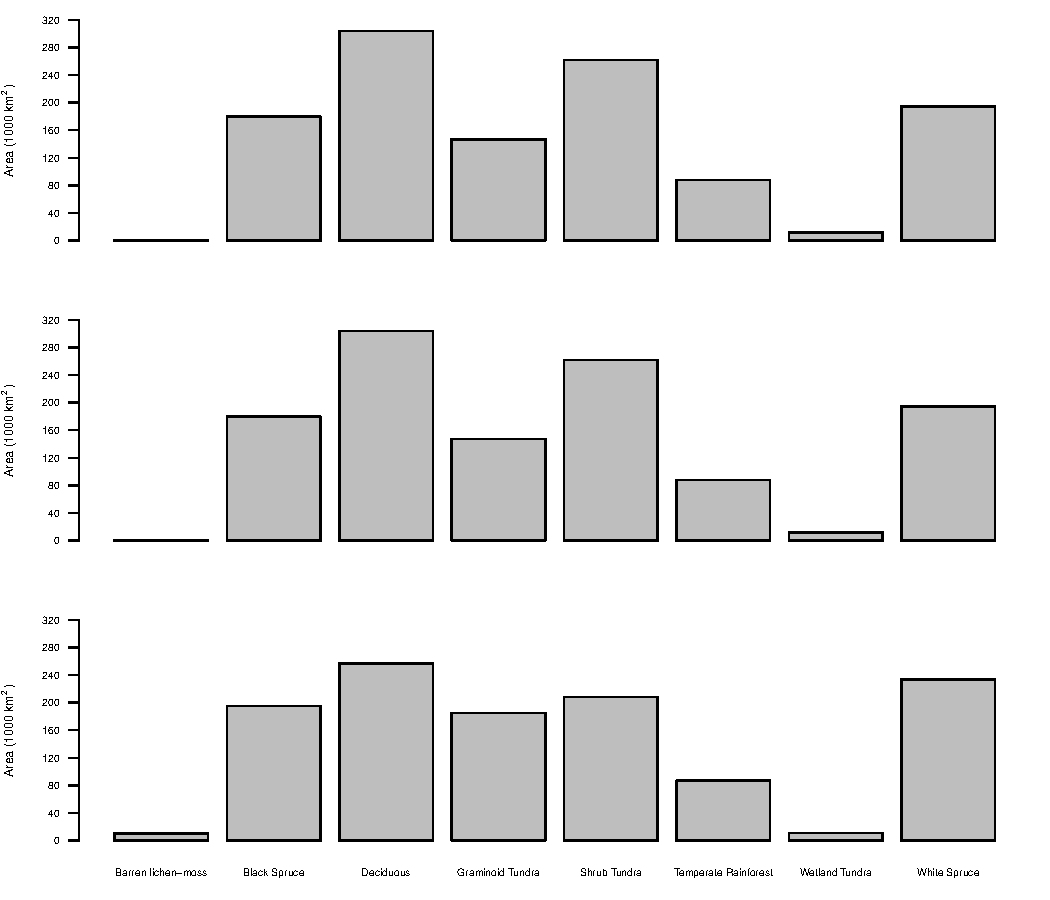
\includegraphics[width=\maxwidth]{figure/baseline_veg_barplot_AK1-1} \caption[Alaska]{Alaska}\label{fig:baseline_veg_barplot_AK1}
\end{figure}


\begin{figure}[H]
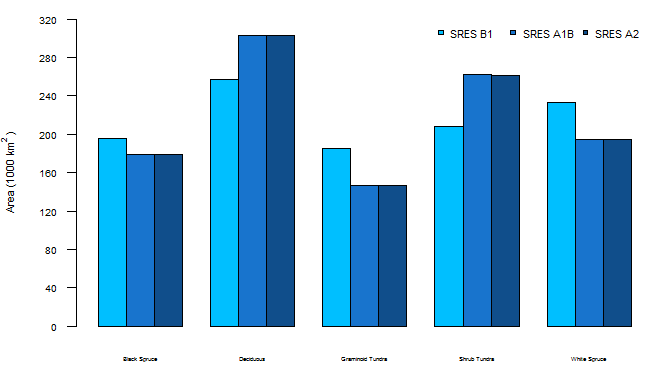
\includegraphics[width=\maxwidth]{figure/baseline_veg_barplot_AK2-1} \caption[Alaska]{Alaska}\label{fig:baseline_veg_barplot_AK2}
\end{figure}



All five following separate LCC graph pairs relate to figure 6.5 (which is just like 6.2) in the original document.
The paired plots are of the same data; the first is like in the original document, but the alternate version may be more readable.
Scenarios are not currently labeled in the original (gray bars) plot version, but they are B1 (top panel), A1B (middle panel), and A2 (bottom panel).
Unlike figure 6.5 (and 6.2), there is a baseline composition for each scenario.
The three baseline panels are plotted separately from the three future net change panels, which are in section 1.2 below.
This uses strictly ALFRESCO output.

\subsubsection{Arctic}
\begin{figure}[H]
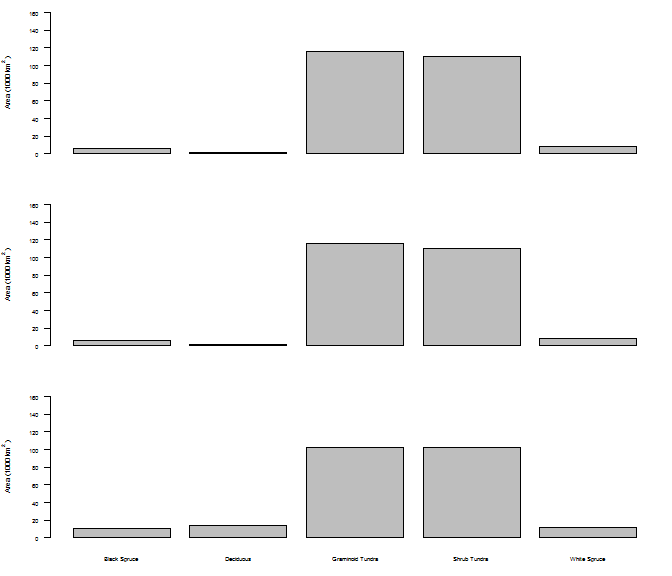
\includegraphics[width=\maxwidth]{figure/baseline_veg_barplot_LCC1a-1} \caption[Arctic]{Arctic}\label{fig:baseline_veg_barplot_LCC1a}
\end{figure}


\begin{figure}[H]
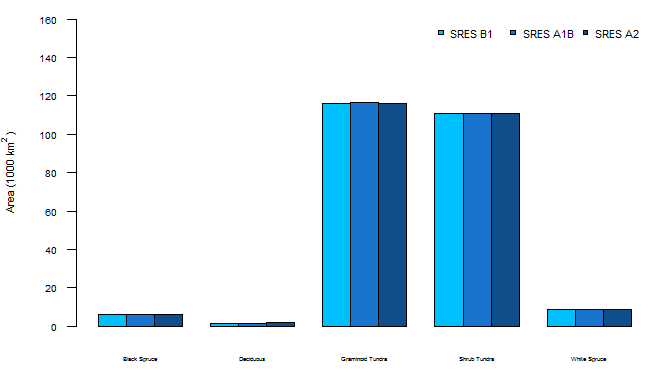
\includegraphics[width=\maxwidth]{figure/baseline_veg_barplot_LCC1b-1} \caption[Arctic]{Arctic}\label{fig:baseline_veg_barplot_LCC1b}
\end{figure}



\subsubsection{North Pacific}
\begin{figure}[H]
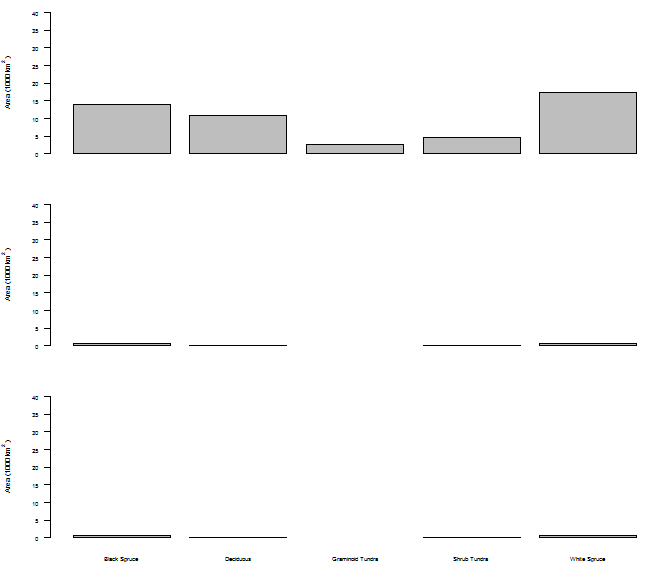
\includegraphics[width=\maxwidth]{figure/baseline_veg_barplot_LCC2a-1} \caption[North Pacific]{North Pacific}\label{fig:baseline_veg_barplot_LCC2a}
\end{figure}


\begin{figure}[H]
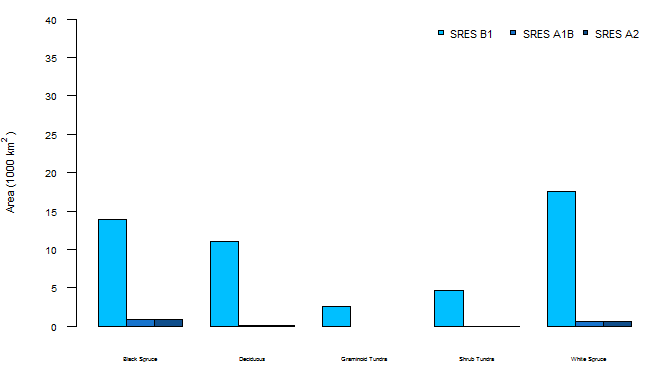
\includegraphics[width=\maxwidth]{figure/baseline_veg_barplot_LCC2b-1} \caption[North Pacific]{North Pacific}\label{fig:baseline_veg_barplot_LCC2b}
\end{figure}



\subsubsection{Northwest Interior Forest North}
\begin{figure}[H]
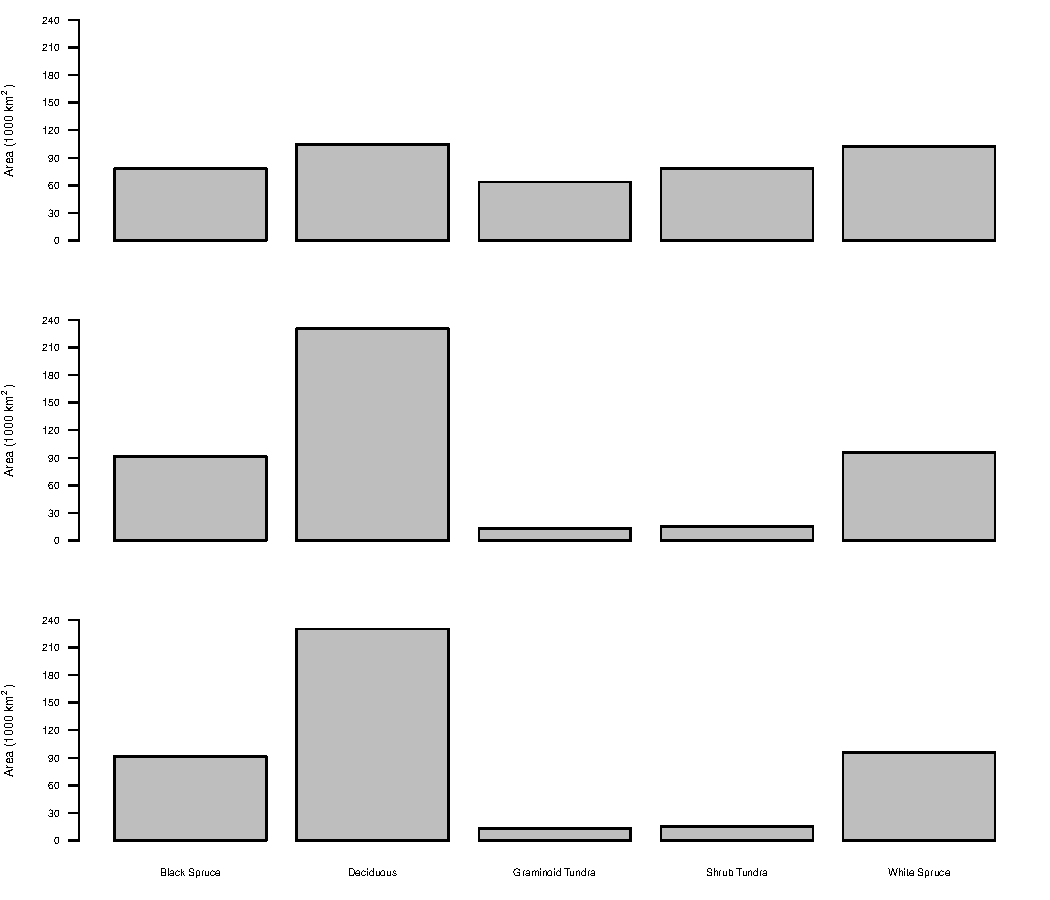
\includegraphics[width=\maxwidth]{figure/baseline_veg_barplot_LCC3a-1} \caption[Northwest Interior Forest North]{Northwest Interior Forest North}\label{fig:baseline_veg_barplot_LCC3a}
\end{figure}


\begin{figure}[H]
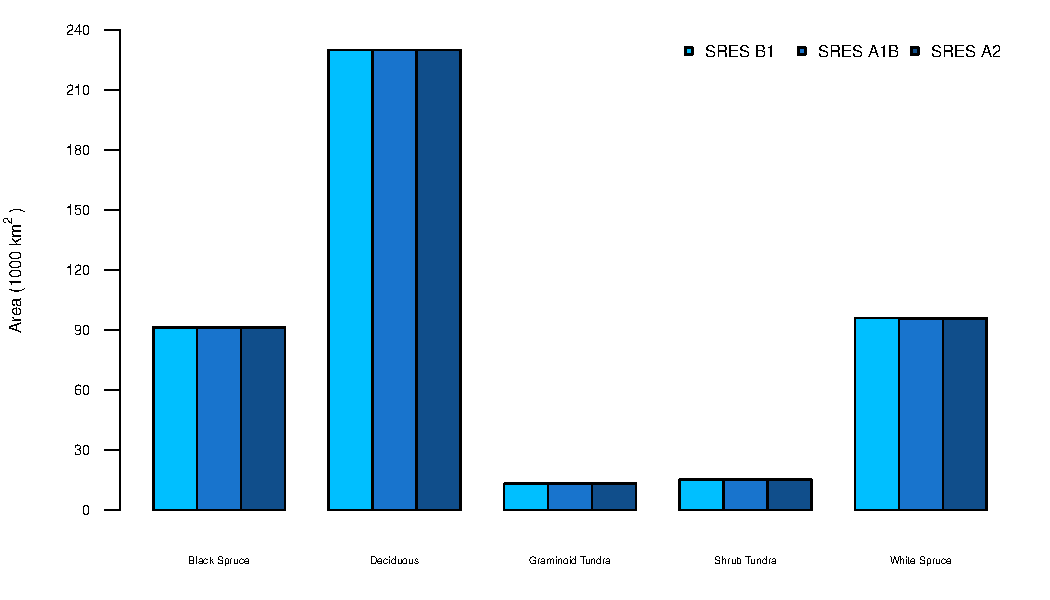
\includegraphics[width=\maxwidth]{figure/baseline_veg_barplot_LCC3b-1} \caption[Northwest Interior Forest North]{Northwest Interior Forest North}\label{fig:baseline_veg_barplot_LCC3b}
\end{figure}



\subsubsection{Northwest Interior Forest South}
\begin{figure}[H]
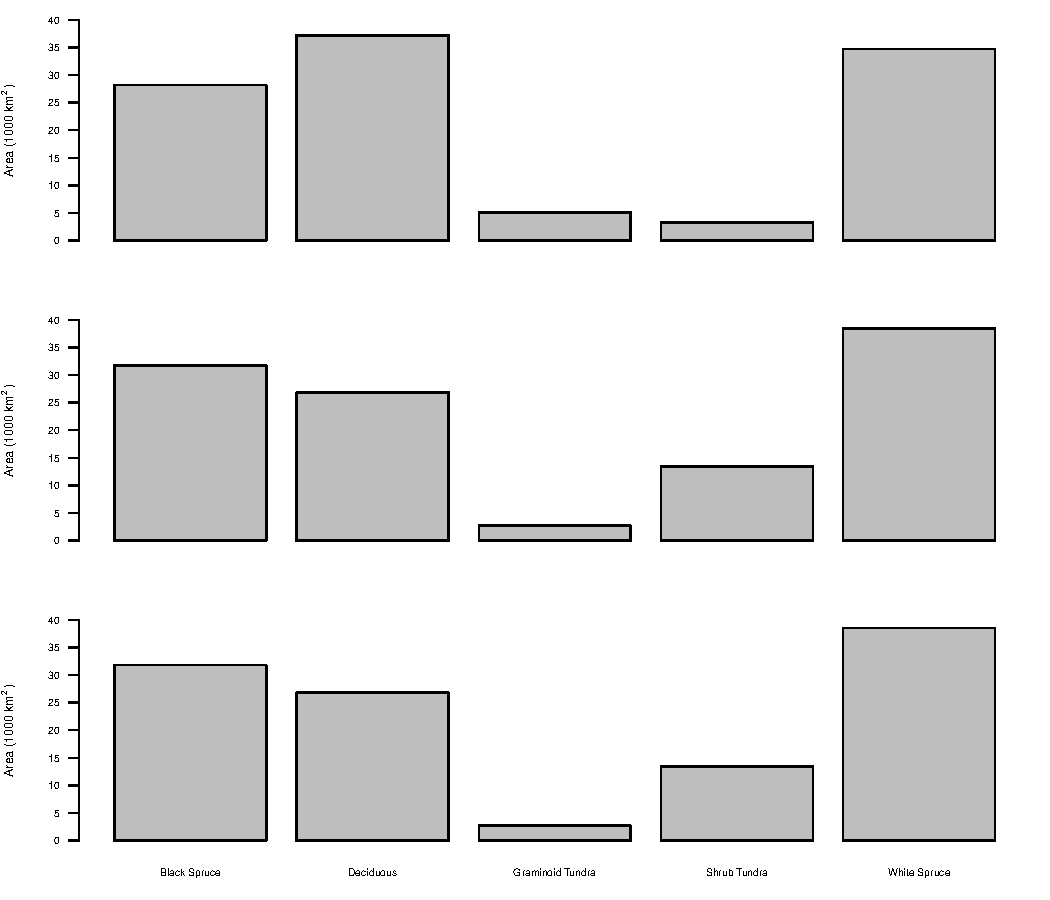
\includegraphics[width=\maxwidth]{figure/baseline_veg_barplot_LCC4a-1} \caption[Northwest Interior Forest South]{Northwest Interior Forest South}\label{fig:baseline_veg_barplot_LCC4a}
\end{figure}


\begin{figure}[H]
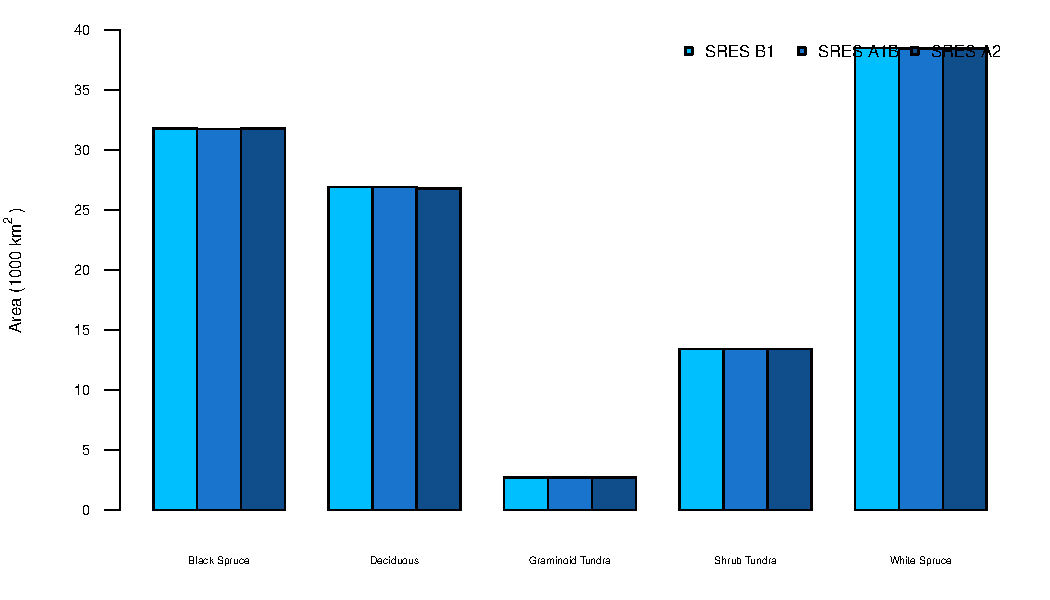
\includegraphics[width=\maxwidth]{figure/baseline_veg_barplot_LCC4b-1} \caption[Northwest Interior Forest South]{Northwest Interior Forest South}\label{fig:baseline_veg_barplot_LCC4b}
\end{figure}



\subsubsection{Western Alaska}
\begin{figure}[H]
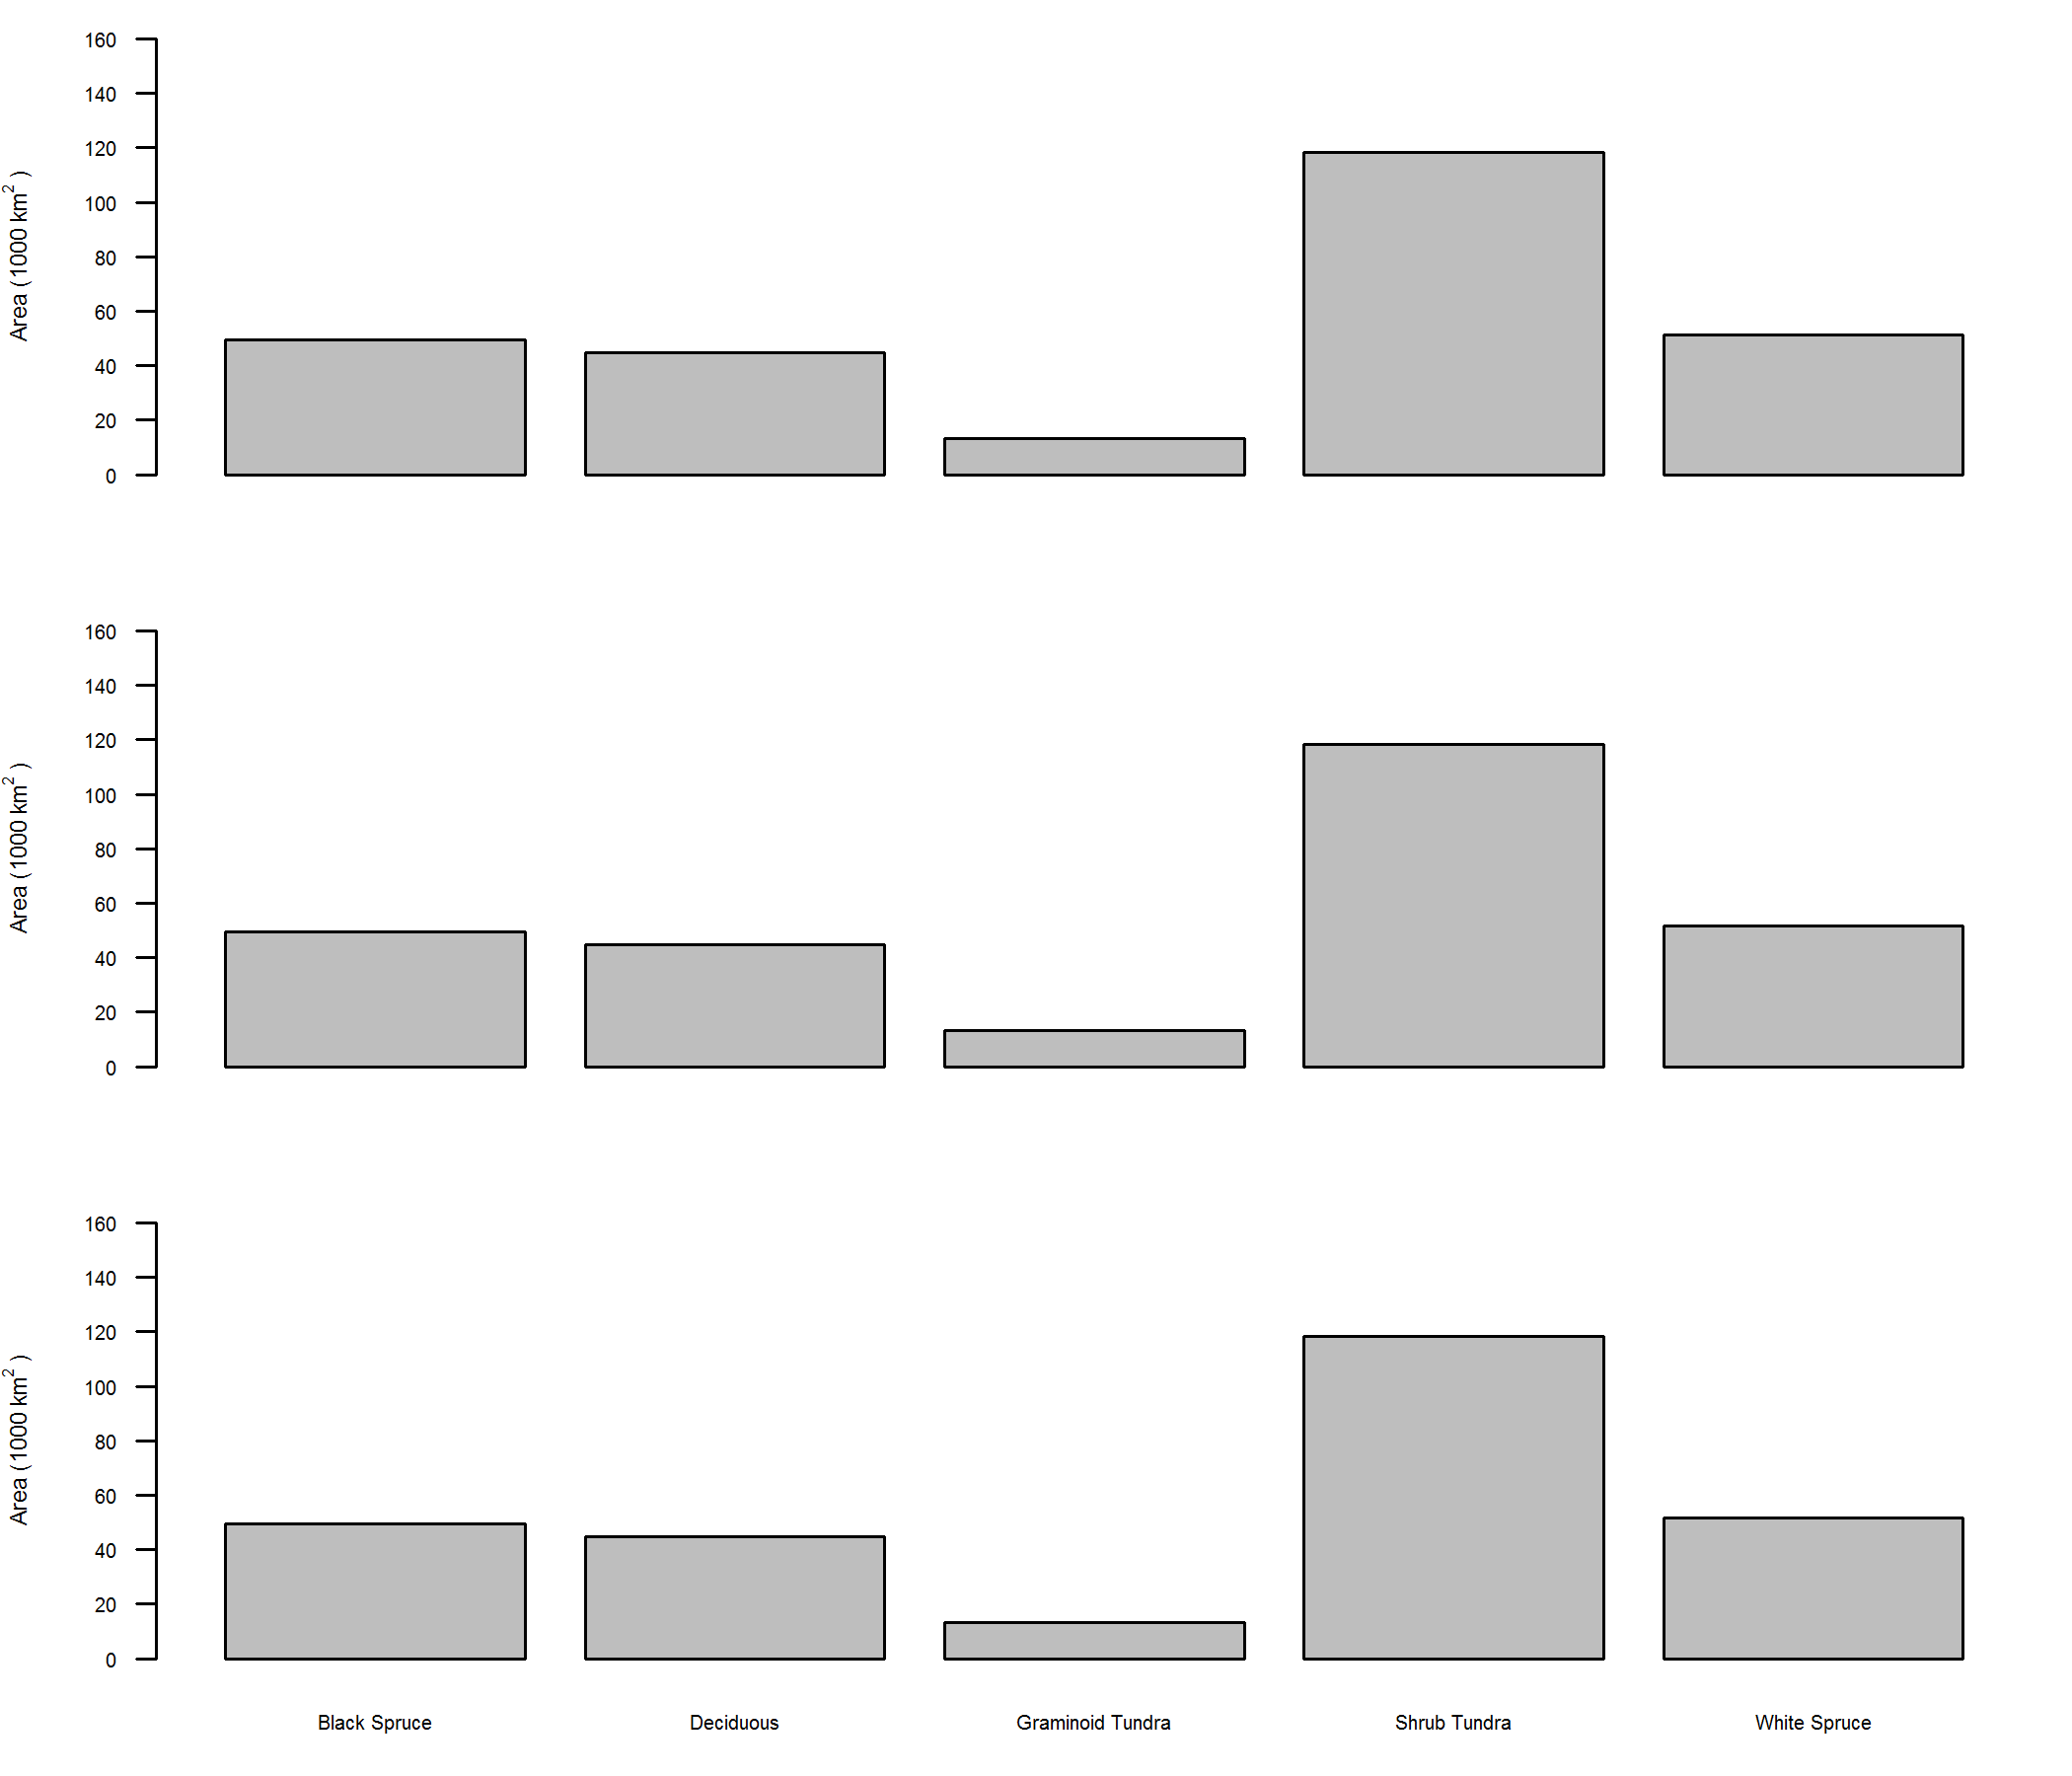
\includegraphics[width=\maxwidth]{figure/baseline_veg_barplot_LCC5a-1} \caption[Western Alaska]{Western Alaska}\label{fig:baseline_veg_barplot_LCC5a}
\end{figure}


\begin{figure}[H]
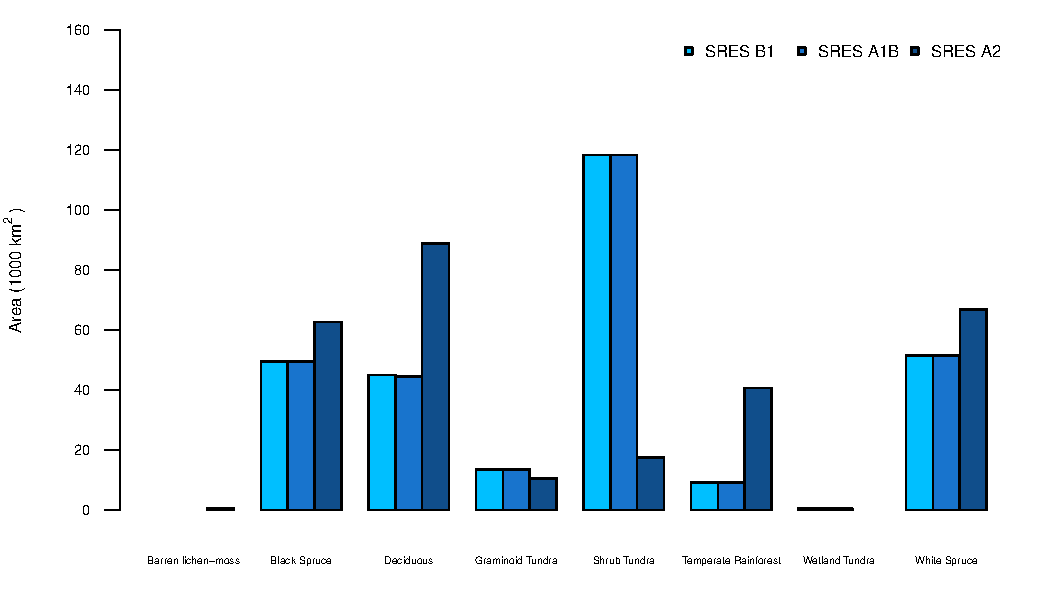
\includegraphics[width=\maxwidth]{figure/baseline_veg_barplot_LCC5b-1} \caption[Western Alaska]{Western Alaska}\label{fig:baseline_veg_barplot_LCC5b}
\end{figure}



\newpage
\subsection{2100 Percent Change by Scenario}
The below graph pair relates to figure 6.2 in the original document, in conjunction with the graph above in section 1.1.1.
The paired plots are of the same data; the first is like in the original document, but the alternate version may be more readable.
Scenarios are not currently labeled in the original (gray bars) plot version, but they are B1 (top panel), A1B (middle panel), and A2 (bottom panel).
This uses strictly ALFRESCO output.

\subsubsection{Alaska}
\begin{figure}[H]
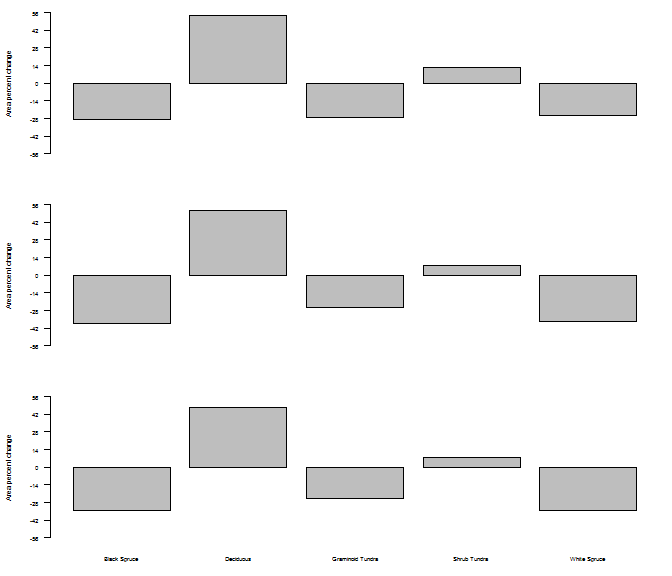
\includegraphics[width=\maxwidth]{figure/veg_change_barplot_AK1-1} \caption[Alaska]{Alaska}\label{fig:veg_change_barplot_AK1}
\end{figure}


\begin{figure}[H]
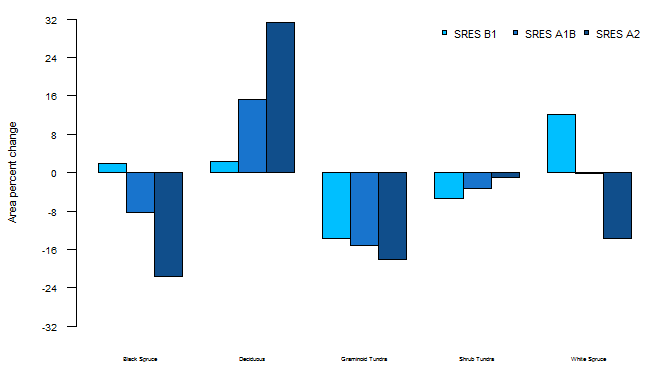
\includegraphics[width=\maxwidth]{figure/veg_change_barplot_AK2-1} \caption[Alaska]{Alaska}\label{fig:veg_change_barplot_AK2}
\end{figure}



All five following separate LCC graph pairs relate to figure 6.5 (which is just like 6.2) in the original document, in conjunction with the respective graph pairs above in sections 1.1.2 - 1.1.6.
The paired plots are of the same data; the first is like in the original document, but the alternate may be more readable.
Unlike figure 6.5 (and 6.2), there is a baseline composition for each scenario.
This uses strictly ALFRESCO output.

\subsubsection{Arctic}
\begin{figure}[H]
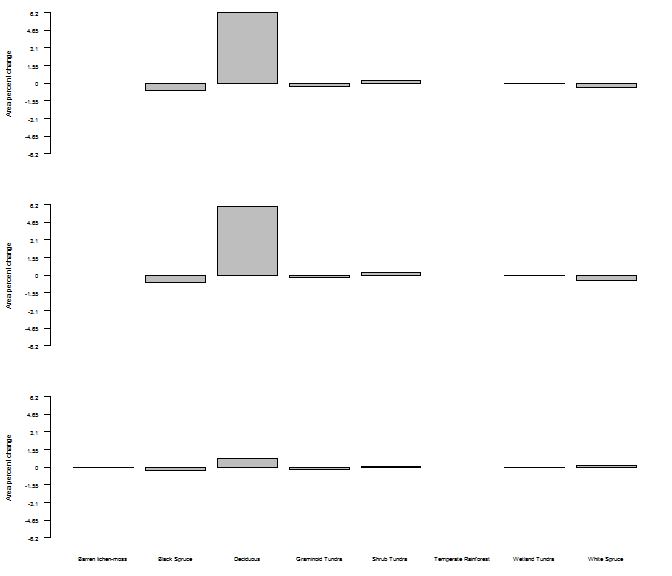
\includegraphics[width=\maxwidth]{figure/veg_change_barplot_LCC1a-1} \caption[Arctic]{Arctic}\label{fig:veg_change_barplot_LCC1a}
\end{figure}


\begin{figure}[H]
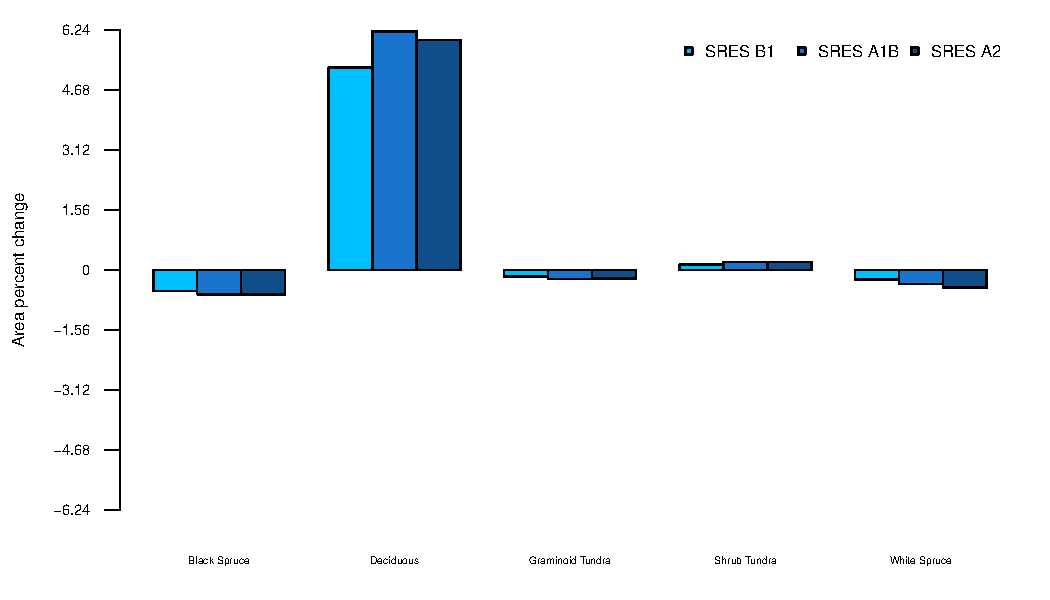
\includegraphics[width=\maxwidth]{figure/veg_change_barplot_LCC1b-1} \caption[Arctic]{Arctic}\label{fig:veg_change_barplot_LCC1b}
\end{figure}



\subsubsection{North Pacific}
\begin{figure}[H]
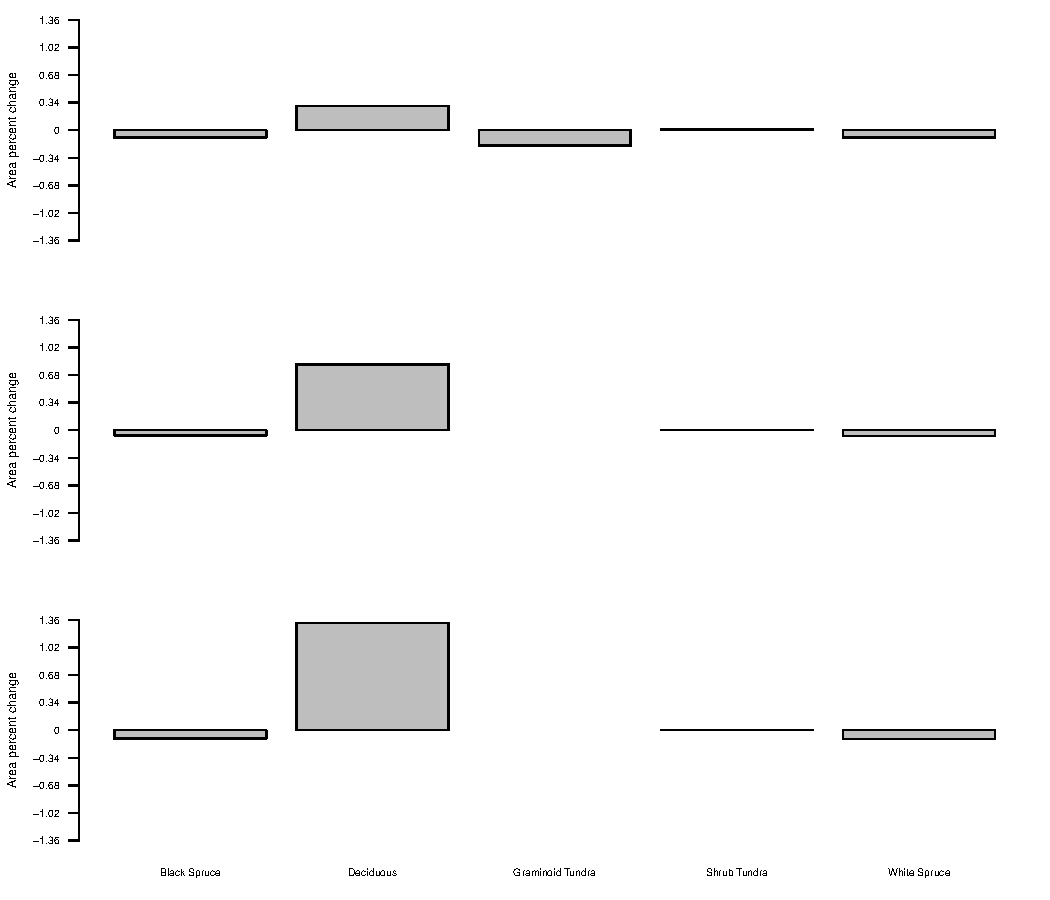
\includegraphics[width=\maxwidth]{figure/veg_change_barplot_LCC2a-1} \caption[North Pacific]{North Pacific}\label{fig:veg_change_barplot_LCC2a}
\end{figure}


\begin{figure}[H]
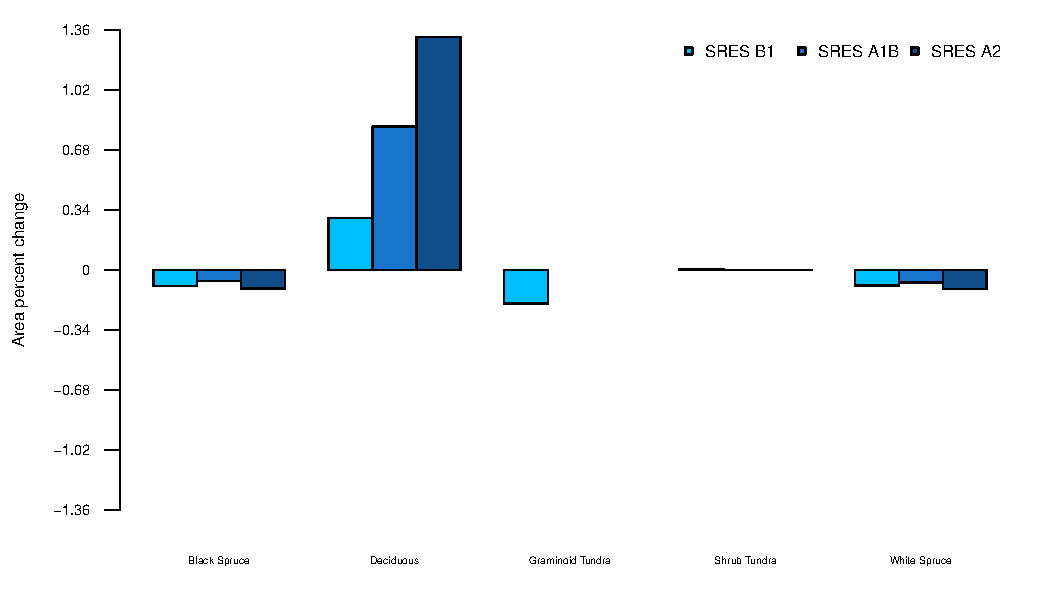
\includegraphics[width=\maxwidth]{figure/veg_change_barplot_LCC2b-1} \caption[North Pacific]{North Pacific}\label{fig:veg_change_barplot_LCC2b}
\end{figure}



\subsubsection{Northwest Interior Forest North}
\begin{figure}[H]
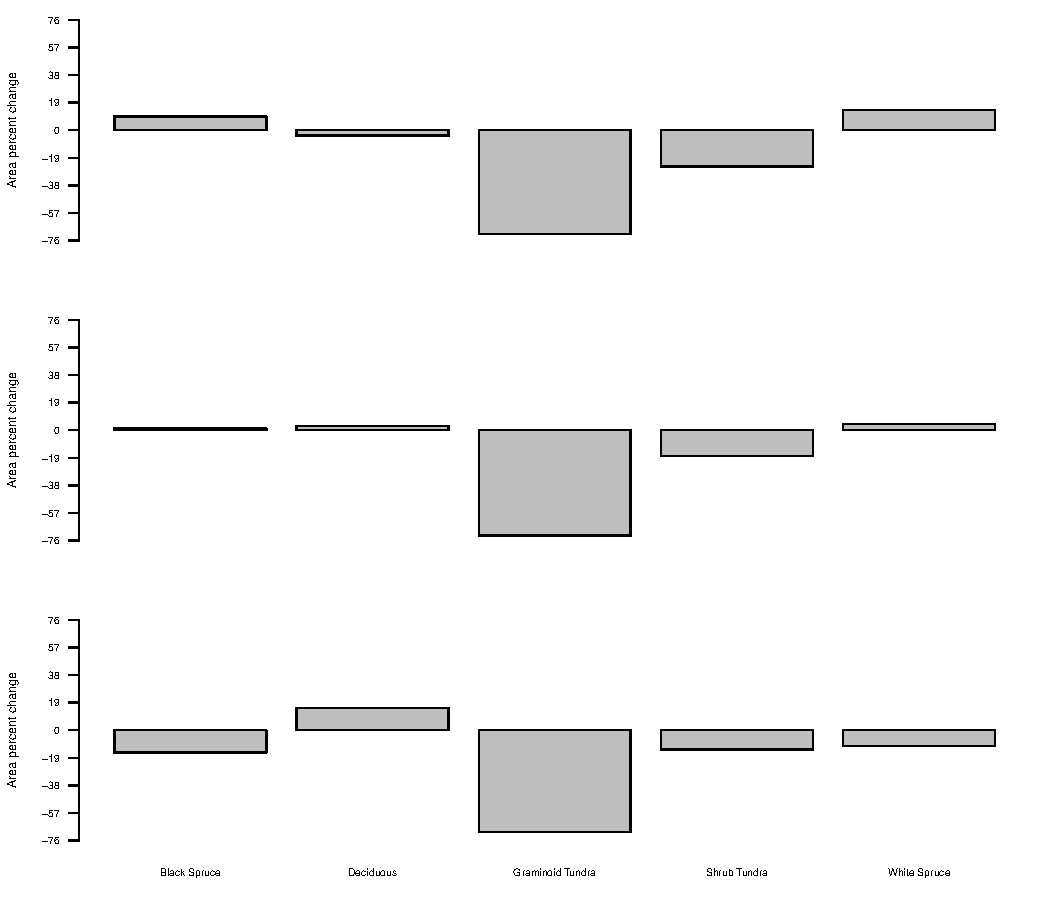
\includegraphics[width=\maxwidth]{figure/veg_change_barplot_LCC3a-1} \caption[Northwest Interior Forest North]{Northwest Interior Forest North}\label{fig:veg_change_barplot_LCC3a}
\end{figure}


\begin{figure}[H]
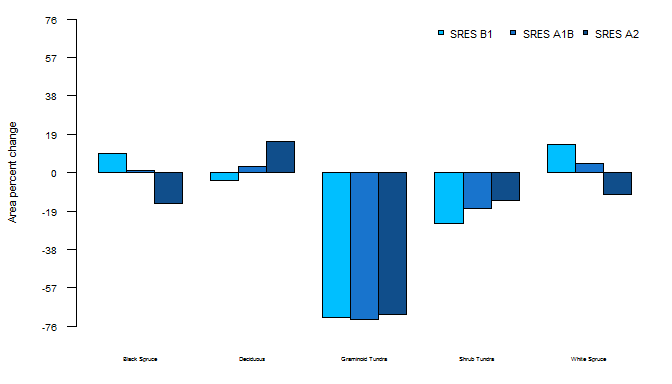
\includegraphics[width=\maxwidth]{figure/veg_change_barplot_LCC3b-1} \caption[Northwest Interior Forest North]{Northwest Interior Forest North}\label{fig:veg_change_barplot_LCC3b}
\end{figure}



\subsubsection{Northwest Interior Forest South}
\begin{figure}[H]
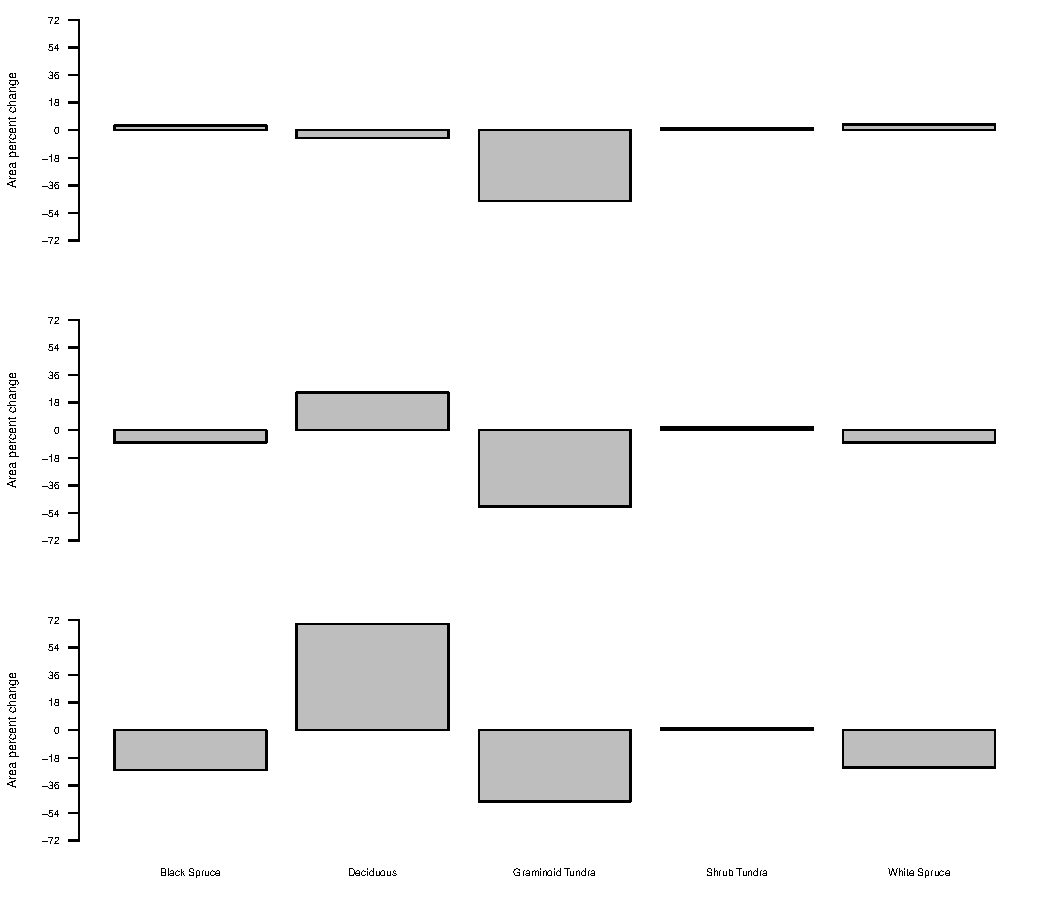
\includegraphics[width=\maxwidth]{figure/veg_change_barplot_LCC4a-1} \caption[Northwest Interior Forest South]{Northwest Interior Forest South}\label{fig:veg_change_barplot_LCC4a}
\end{figure}


\begin{figure}[H]
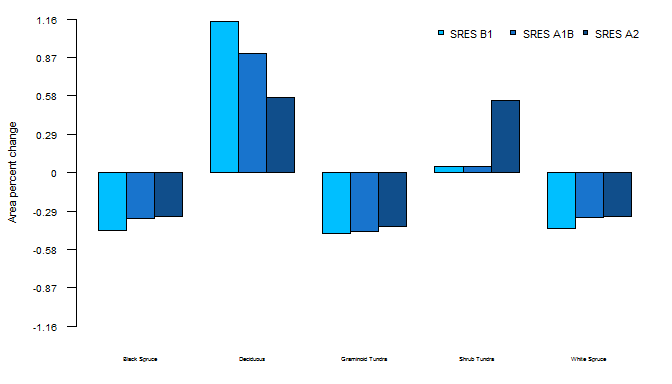
\includegraphics[width=\maxwidth]{figure/veg_change_barplot_LCC4b-1} \caption[Northwest Interior Forest South]{Northwest Interior Forest South}\label{fig:veg_change_barplot_LCC4b}
\end{figure}



\subsubsection{Western Alaska}
\begin{figure}[H]
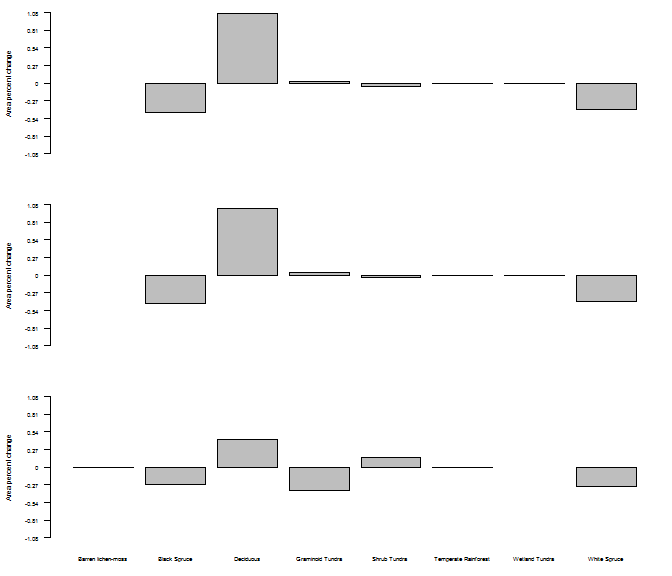
\includegraphics[width=\maxwidth]{figure/veg_change_barplot_LCC5a-1} \caption[Western Alaska]{Western Alaska}\label{fig:veg_change_barplot_LCC5a}
\end{figure}


\begin{figure}[H]
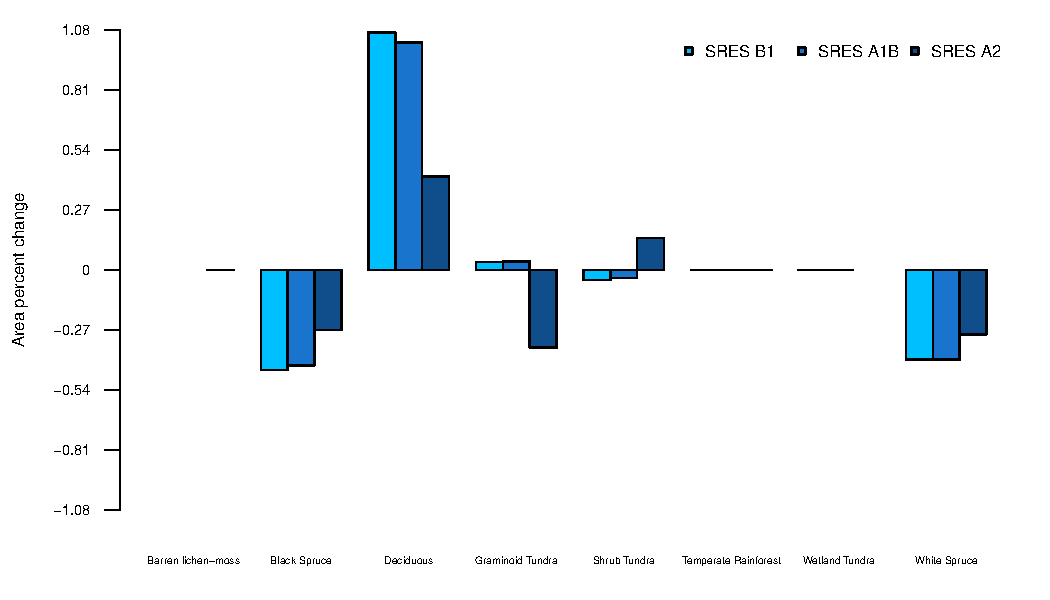
\includegraphics[width=\maxwidth]{figure/veg_change_barplot_LCC5b-1} \caption[Western Alaska]{Western Alaska}\label{fig:veg_change_barplot_LCC5b}
\end{figure}



\end{document}
